\renewcommand{\theequation}{\theenumi}
\begin{enumerate}[label=\thesection.\arabic*.,ref=\thesection.\theenumi]
\numberwithin{equation}{enumi}

\item Let us take vertically upward direction as +ve y-axis and west to east direction as +ve x-axis.The woman experiences rain in the direction of the relative velocity of the rain wrt her own velocity.
The velocity of rain = $\vec{v_r} = \myvec{0\\-35}$
\newline
The velocity of woman = $\vec{v_w} = \myvec{-12\\0}$
\newline
relative velocity of rain wrt woman is given as
\begin{align}
\vec{v_{r_w}} =\vec{v_r}- \vec{v_w}
\implies \myvec{12\\-35}
\end{align}
She must hold the umbrella opposite to the direction of rain she experiences.So the woman must hold the umbrella along the direction of $-\vec{v_{r_w}}$
So the woman must hold the umbrella forward at an angle $\theta$ to the vertical where
\begin{align}
\theta={\tan}^{-1}\brak{\frac{12}{35}}
\end{align}
The following python code generates figure \ref{fig:rain} which illustrates the velocities $\vec{v_r},\vec{v_w},\vec{v_{r_w}}$
%
\begin{lstlisting}
codes/line/rain/rain.py
\end{lstlisting}
\begin{figure}[!ht]
\centering
\includegraphics[width=\columnwidth]{./codes/line/rain/pyfigs/rain.eps}
\caption{Direction of umbrella}
\label{fig:rain}
\end{figure}
\end{enumerate}
